% 92-22(92쪽) — 한 변의 길이가 6 인 정사각형 ABCD 와 한 변의 길이가 2 인 정사각형 CEFG(원문 「오른쪽 그림」). 스캔 화질이 낮아 TikZ 로 다시 그림.
% 라벨은 원문 것만: 꼭짓점 A·B·C·D·E·F·G, 길이 6·2, 각 θ. DG·BE 의 값(답)은 그림에 적지 않는다.
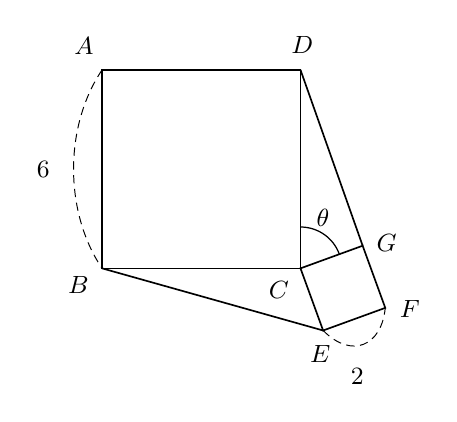
\begin{tikzpicture}[line width=0.6pt, x=0.42cm, y=0.42cm]
  \coordinate (A) at (0,6);
  \coordinate (B) at (0,0);
  \coordinate (C) at (6,0);
  \coordinate (D) at (6,6);
  \coordinate (G) at (7.879,0.684);
  \coordinate (F) at (8.563,-1.195);
  \coordinate (E) at (6.684,-1.879);
  \draw (A) -- (B) -- (C) -- (D) -- cycle;
  \draw (C) -- (E) -- (F) -- (G) -- cycle;
  \draw (D) -- (G);
  \draw (B) -- (E);
  % 각 θ 표시
  \draw[line width=0.45pt] ([shift={(20:1.25)}]C) arc [start angle=20, end angle=90, radius=1.25];
  % 길이 표시의 점선 호
  \draw[densely dashed, line width=0.35pt] (A) .. controls (-1.15,4.3) and (-1.15,1.7) .. (B);
  \draw[densely dashed, line width=0.35pt] (E) .. controls (7.55,-2.75) and (8.45,-2.35) .. (F);
  \node[font=\small, anchor=south east] at (0.05,6.15) {$\pt{A}$};
  \node[font=\small, anchor=north east] at (-0.10,0.05) {$\pt{B}$};
  \node[font=\small, anchor=north east] at (5.95,-0.10) {$\pt{C}$};
  \node[font=\small, anchor=south] at (6.05,6.18) {$\pt{D}$};
  \node[font=\small, anchor=north] at (6.60,-2.02) {$\pt{E}$};
  \node[font=\small, anchor=west] at (8.70,-1.22) {$\pt{F}$};
  \node[font=\small, anchor=west] at (8.00,0.76) {$\pt{G}$};
  \node[font=\small, anchor=east] at (-1.28,3.0) {$6$};
  \node[font=\small, anchor=north] at (7.72,-2.72) {$2$};
  \node[font=\small, anchor=south west] at (6.18,0.95) {$\theta$};
\end{tikzpicture}
